\documentclass[twoside,10pt]{article}
\usepackage{shlists}
\usepackage[applemac]{inputenc}
\usepackage[spanish]{babel}
\usepackage[T1]{fontenc}


\usepackage{multicol}
\usepackage{picinpar}

\usepackage{url}
\newcommand{\surl}[1]{{\small\url{#1}}}

\newcounter{vol}
\newcounter{num}
\newcounter{anyo}
\setcounter{vol}{9}
\setcounter{num}{2}
\setcounter{anyo}{2016}
\newcommand{\mes}{Mayo}
\usepackage{revisionNLcol}


\title{\ \\ Docencia 2.0\\ \large Juan Juli\'{a}n Merelo, Fernando Tricas}
\author{\LARGE Lenguajes de programaci�n: �uno, ninguno o todos?}

\date{}

\AutTit{Docencia 2.0}

\begin{document}
\addtocounter{page}{2}

\maketitle
\vspace*{-5ex}

\begin{multicols}{2}

Si hay un tema universal en la inform�tica son los lenguajes de
programaci�n. Desde los niveles m�s bajos de la arquitectura a los m�s
altos, la forma universal en la que el ser humano se comunica con un
ordenador es un lenguaje. Los lenguajes suelen tener una serie de
caracter�sticas comunes: una sintaxis r�gida, implementaciones libres y
una evoluci�n continua.

En esta �ltima caracter�stica est� uno de los problemas. El lenguaje
que ense�aste en primero puede no parecerse en nada al que usar�s en
el trabajo fin de grado. Pero si consideramos que la evoluci�n
individual est� acompa�ada de una evoluci�n colectiva de los tipos de
lenguajes que se usan y que, por tanto, se necesitan no ya para
conseguir un puesto de trabajo, sino siquiera para poder trabajar en
un entorno de computaci�n determinado, la elecci�n de un lenguaje de
programaci�n para una asignatura o para una carrera entera se
convierte en una tarea ardua o imposible.

Porque, seamos pr�cticos, elegir un solo lenguaje para regirlos a
todos es imposible en nuestro pa�s. Nuestra idiosincrasia impedir�a
que m�s de dos personas se pusieran de acuerdo en qu� lenguaje usar
desde primero a cuarto, y en el caso improbable de que un {\em ukase}
de la superioridad impusiera uno, esa misma idiosincrasia har�a que el
profesor de pr�cticas de 3� usara eventualmente el que le viniera en
gana. 

Descartada esa opci�n.

%--------------------------
\noindent\rule{86mm}{1pt}
\vspace{1ex} {\small{\begin{window}[0,r,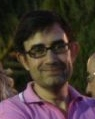
\includegraphics[width = 27mm]{JJM.jpg},] 
\noindent\emph{JJ Merelo} es catedr\'{a}tico de Universidad
en el \'area de Arquitectura y Tecnolog\'{\i}a de Computadores, y
actualmente director de la Oficina de Software Libre de la UGR.
Mantiene un blog desde el a\~no 2002, y lo ha utilizado en clase desde
el a\~no 2004; tambi\'en wikis, agregadores y repositorios de c\'odigo
como herramientas docente. \'{U}ltimamente le ha dado por el \textsl{flipped
learning}, de lo que se informar\'{a} debidamente en esta columna.
\end{window}}}

\medskip

{\small{\begin{window}[0,r,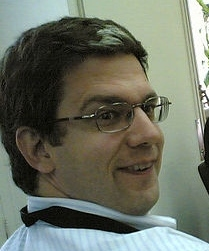
\includegraphics[width = 27 mm]{FTricas1.jpg},]
		\noindent \emph{Fernando Tricas Garc\'{\i}a} es profesor
		titular de Lenguajes y Sistemas Inform\'{a}ticos del Departamento
		de Inform\'{a}tica e Ingenier\'{\i}a de Sistemas de la Universidad de
		Zaragoza.  Empez\'{o} a estudiar la blogosfera casi cuando a\'{u}n no
		exist\'{\i}a (all\'{a} por el a\~{n}o 2002) y a tratar de integrarla en los
		cursos y tareas docentes un poco despu\'{e}s.  Ha impartido
		numerosas charlas relacionadas con el tema de la Web 2.0, 

		internet y universidad,\ldots\ 
		Es actualmente Vicerrector de Tecnolog\'{\i}as de la Informaci\'{o}n y
de la Comunicaci\'{o}n.   
		\end{window}}}
%-------------------------------------------------


\noindent  
\bigskip

\noindent\emph{Todas las columnas de la serie Docencia 2.0
pueden descargarse en formato LaTeX desde
\surl{https://github.com/ReVision-Docencia-20/Columnas}}

\noindent\rule{90mm}{1pt}

{\small \noindent\copyright 2016 JJ. Merelo, F. Tricas. Este art\'{\i}culo es de acceso libre distribuido bajo los t\'{e}rminos
de la Licencia Creative Commons de Atribuci\'{o}n, que permite copiar,
distribuir y comunicar p\'{u}blicamente la obra en cualquier medio, s\'{o}lido
o electr\'{o}nico, siempre que se acrediten a los autores y fuentes
originales}

\end{multicols}
\end{document}
